\documentclass[]{article}

% Imported Packages
%------------------------------------------------------------------------------
\usepackage{amssymb}
\usepackage{amstext}
\usepackage{amsthm}
\usepackage{amsmath}
\usepackage{enumerate}
\usepackage{fancyhdr}
\usepackage[margin=1in]{geometry}
\usepackage{graphicx}
%\usepackage{extarrows}
\usepackage{setspace}
\usepackage{float}
\usepackage{array}
%------------------------------------------------------------------------------

% Header and Footer
%------------------------------------------------------------------------------
\pagestyle{plain}  
\renewcommand\headrulewidth{0.4pt}                                      
\renewcommand\footrulewidth{0.4pt}                                    
%------------------------------------------------------------------------------

% Title Details
%------------------------------------------------------------------------------
\title{Deliverable \#3 Template}
\author{Keyur, Joshua, Abdullah, Justin, Bilal, Shaad}
\date{}                               
%------------------------------------------------------------------------------

% Document
%------------------------------------------------------------------------------
\begin{document}

\maketitle	

\section{Introduction}
\label{sec:introduction}
% Begin Section

\subsection{Purpose}
\label{sub:purpose}
The purpose of this document is to provide the software development team an overall guide to the architecture of this project. This document is published to outline all the parts of the MovieFinder software and to be a reference point for the team developing the application. The intended audience of this document are the software development team of MovieFinder, as well as  the professor and teaching assistants reviewing this design document.

\subsection{System Description}
\label{sub:system_description}
The application MovieFinder has three main `screens.' When the application is launched, the user is displayed the main menu, where they can enter the information they know about the movie. Once they submit that information, the server will then recieve the query and process the query. Once the application has processed the results from the agents, the results will be sent to the client, and be displayed on the results menu. Once on the results menu, users will have the option of sorting the results by certain qualities including but not limited to rating or release date. Users can then choose a single movie to receive more information about. The server will use a universal movie database to get the information. This information takes users to the third screen, which is the information menu.

\subsection{Overview}
\label{sub:overview}
This document contains state charts for the controller classes of the application. These state charts provide a full description of the behaviour of the controller classes. Next, the design document contains the sequence diagrams. These sequence diagrams illustrate the flow of information from class to class under different scenarios. Lastly, this document shows the detailed class diagrams required to develop the MovieFinder. The detailed class diagrams provide a blueprint for the classes and their methods, as well as how they are connected to each other.


\section{State Charts for Controller Classes}
\label{sec:state_charts_for_controller_classes}
% Begin Section
\begin{figure}[H]
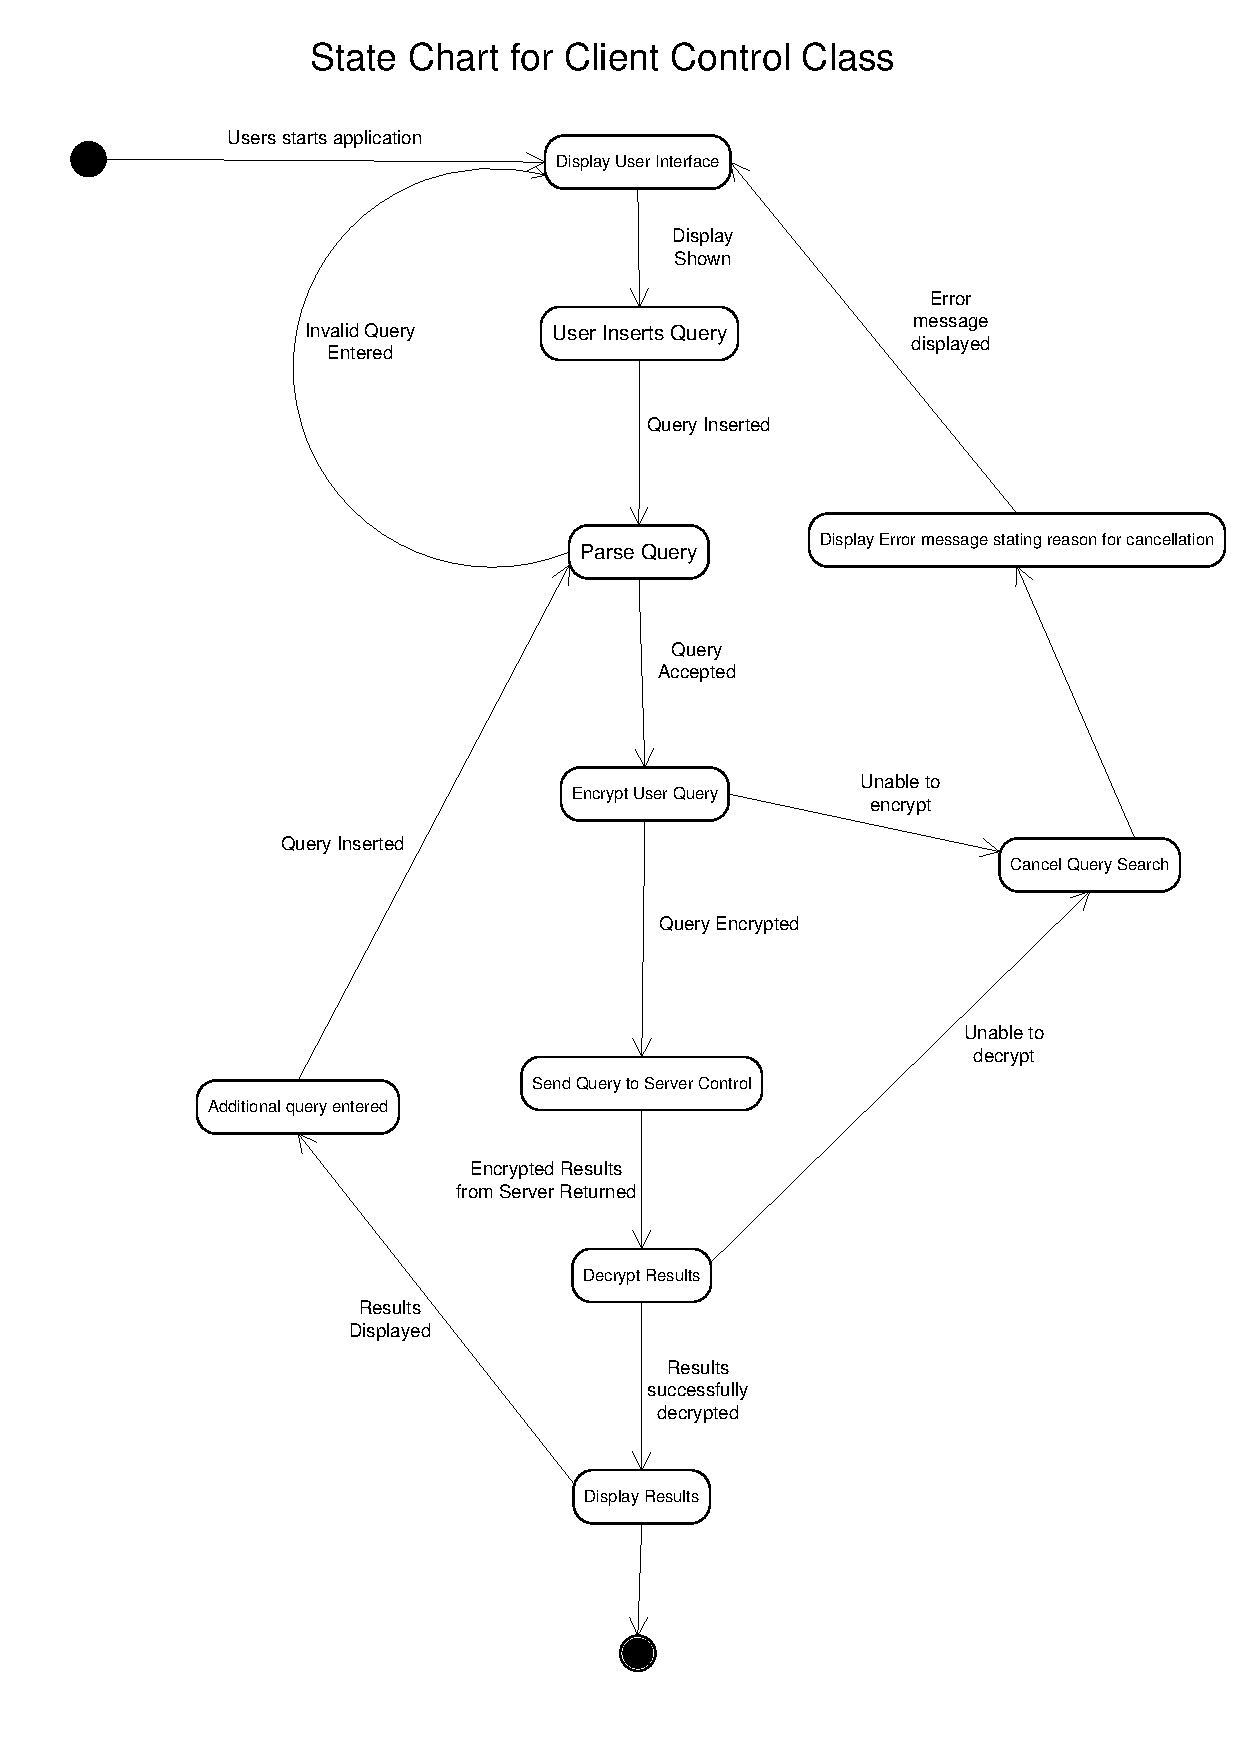
\includegraphics[width=\textwidth]{state-chart-client}
\centering
\caption{State chart for client}
\end{figure}

\begin{figure}[H]
\includegraphics[width=\textwidth]{state-chart-server}
\centering
\caption{State chart for server}
\end{figure}
% End Section

\section{Sequence Diagrams}
\label{sec:sequence_diagrams}
\begin{figure}[H]
	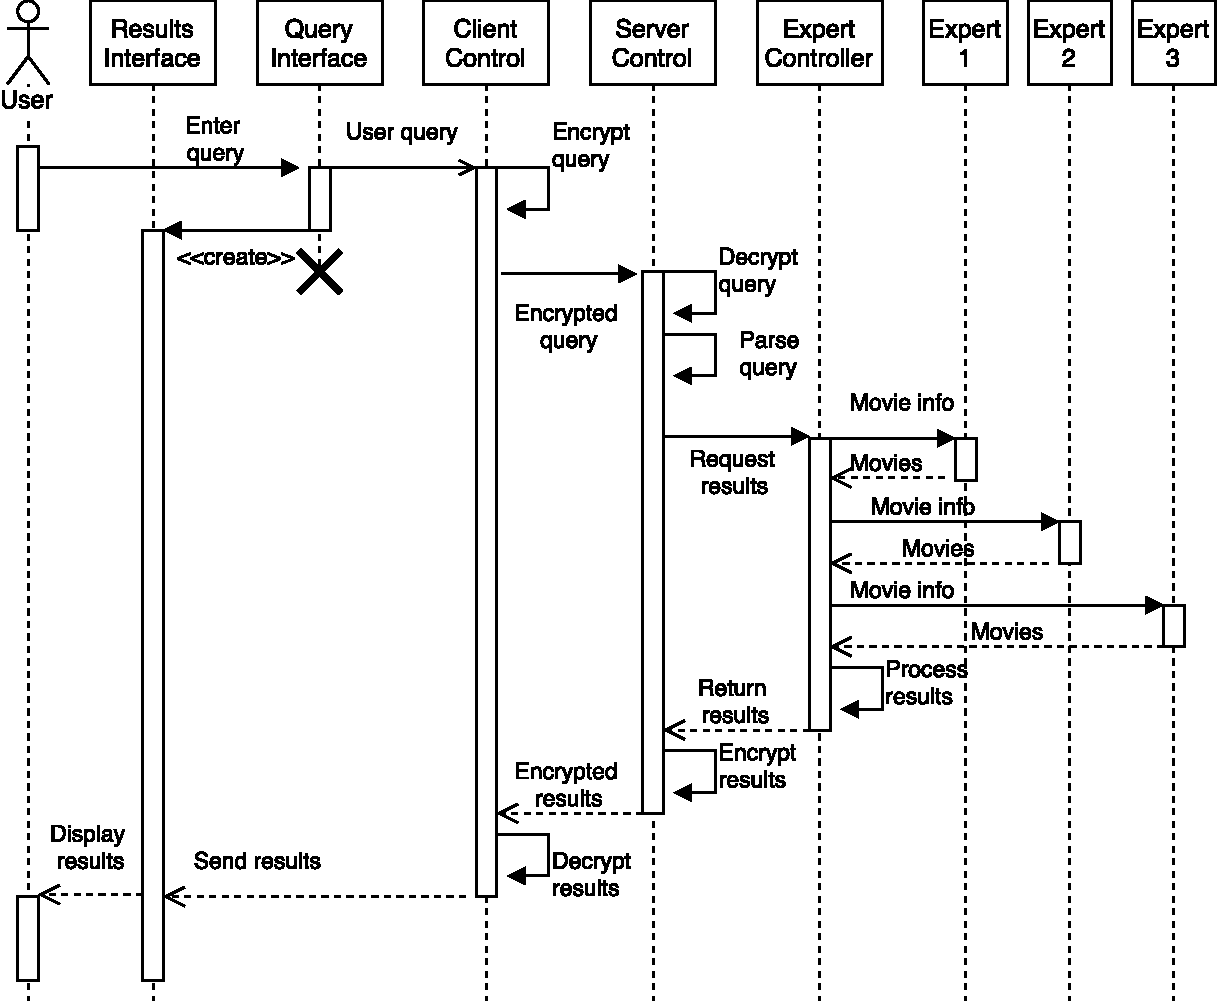
\includegraphics[width=\textwidth]{SD1}
	\centering
	\caption{Sequence diagram for entering a query}
\end{figure}

\begin{figure}[H]
	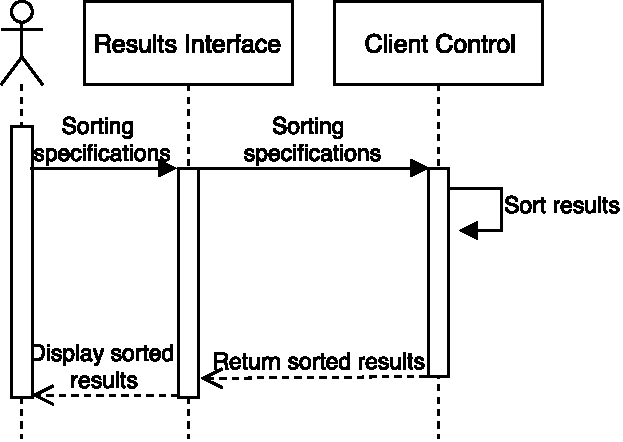
\includegraphics[width=\textwidth]{SD2}
	\centering
	\caption{Sequence diagram for sorting the results}
\end{figure}

\begin{figure}[H]
	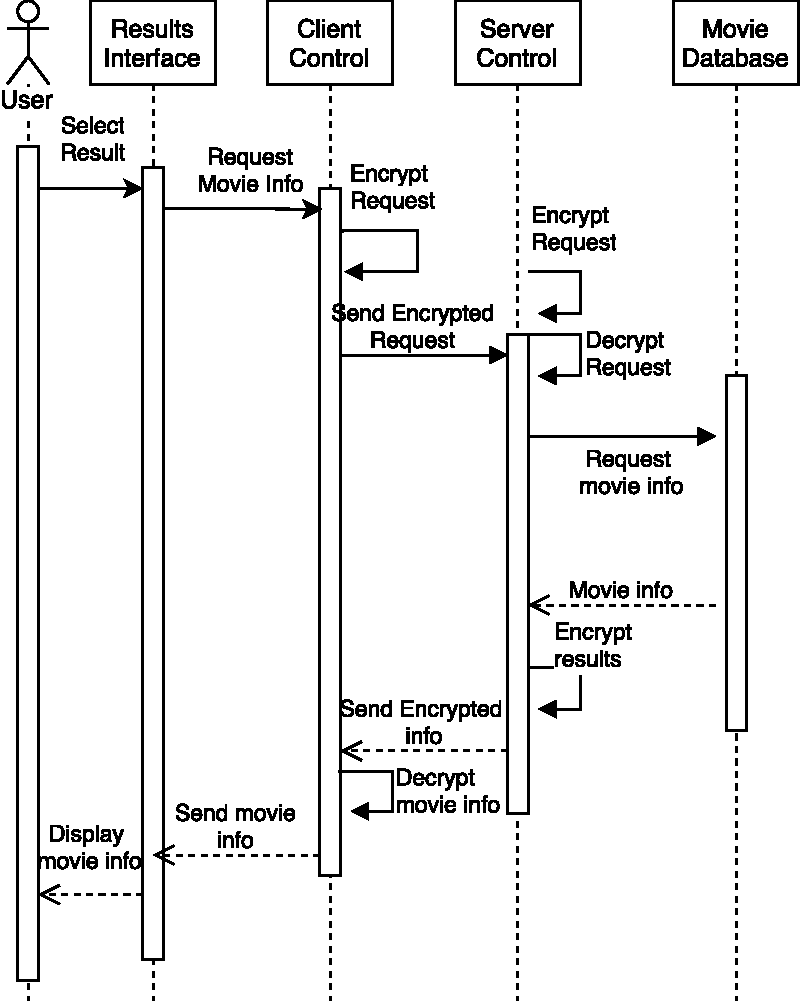
\includegraphics[width=\textwidth]{SD3}
	\centering
	\caption{Sequence diagram for viewing individual movie information}
\end{figure}

\section{Detailed Class Diagram}
\label{sec:detailed_class_diagram}
% Begin Section
\begin{table}[H]
\centering % centers tables in page
\begin{tabular}{|>{\centering\arraybackslash}p{10cm}|} % centers text in table while specifying table width
% use immediately preceding column specifier
\hline
Client Control\\
\hline
\begin{itemize}
\item[-] clientID: int
\item[-] clientquery(): Object
\item[-] queryResponse(): Object
\end{itemize}
\\
\hline
\begin{itemize}
\item[+] constructor()
\item[+] init()
\item[+] listener(): void
\item[+] recordQuery(q: Query): void
\item[+] sendQuery():  Object
\end{itemize}
\\
\hline
\end{tabular}
\end{table}
%
\begin{table}[H]
\centering
\begin{tabular}{|>{\centering\arraybackslash}p{10cm}|}
\hline
Result Interface\\
\hline
\begin{itemize}
\item[-] query: String
\end{itemize}
\\
\hline
\begin{itemize}
\item[+] constructor()
\item[+] setResult(q: String): void
\item[+] getResult(l: String): String
\item[+] displayResult(): void
\item[+] removeResult(): void
\end{itemize}
\\
\hline
\end{tabular}
\end{table}
%
\begin{table}[H]
\centering
\begin{tabular}{|>{\centering\arraybackslash}p{10cm}|}
\hline
Query Form\\
\hline
\begin{itemize}
\item[-] selection: Object
\end{itemize}
\\
\hline
\begin{itemize}
\item[+] constructor()
\item[+] getResult(result: Object): void
\item[+] actionPerformed(event: Object): void
\item[+] mouseClicked(event: Object): void
\item[+] sendResult(result: Object): Object
\end{itemize}
\\
\hline
\end{tabular}
\end{table}
%
\begin{table}[H]
\centering
\begin{tabular}{|>{\centering\arraybackslash}p{10cm}|}
\hline
Server Control\\
\hline
\begin{itemize}
\item[-] expertList: Expert[3] = [expert1, expert2, expert3]
\item[-] clientID: int[] = null
\item[-] clientQuery: object[] = null
\item[-] queryResponse: object[] = null

\end{itemize}
\\
\hline
\begin{itemize}
\item[+] contructor()
\item[+] init()
\item[+] listen()
\item[+] readQuery(Query query): object
\item[+] sendResult(Object object)
\item[+] lockExpert(String expert)
\end{itemize}
\\
\hline
\end{tabular}
\end{table}
%
\begin{table}[H]
\centering
\begin{tabular}{|>{\centering\arraybackslash}p{10cm}|}
\hline
Expert 1 Control\\
\hline
%\begin{itemize}
%\item[-] private
%\end{itemize}
%\\
%\hline
\begin{itemize}
\item[+] constructor()
\item[+] init()
\item[+] update()
\item[+] search(Object query): Object[]
\item[+] addItem(Object newObject)
\item[+] removeItem(Object oldObject): Object
\end{itemize}
\\
\hline
\end{tabular}
\end{table}
%
\begin{table}[H]
\centering
\begin{tabular}{|>{\centering\arraybackslash}p{10cm}|}
\hline
Expert 1 Database\\
\hline
\begin{itemize}
\item[-] movieList: String[] = null
\item[-] paramterList: enumerate = 1..N
\item[-] parameterData1: Object[] = null
\item[-] paramterDataN: Object[] = null
\end{itemize}
\\
\hline
\begin{itemize}
\item[+] constructor()
\item[+] deconstructor()
\item[+] init()
\end{itemize}
\\
\hline
\end{tabular}
\end{table}
%
\begin{table}[H]
\centering
\begin{tabular}{|>{\centering\arraybackslash}p{10cm}|}
\hline
Expert 2 Control\\
\hline
%\begin{itemize}
%\item[-] private
%\end{itemize}
%\\
%\hline
\begin{itemize}
\item[+] constructor()
\item[+] init()
\item[+] update()
\item[+] search(Object query): Object[]
\item[+] addItem(Object newObject)
\item[+] removeItem(Object oldObject): Object
\end{itemize}
\\
\hline
\end{tabular}
\end{table}
%
\begin{table}[H]
\centering
\begin{tabular}{|>{\centering\arraybackslash}p{10cm}|}
\hline
Expert 2 Database\\
\hline
\begin{itemize}
\item[-] movieList: String[] = null
\item[-] paramterList: enumerate = 1..N
\item[-] parameterData1: Object[] = null
\item[-] paramterDataN: Object[] = null
\end{itemize}
\\
\hline
\begin{itemize}
\item[+] constructor()
\item[+] deconstructor()
\item[+] init()
\end{itemize}
\\
\hline
\end{tabular}
\end{table}
%
\begin{table}[H]
\centering
\begin{tabular}{|>{\centering\arraybackslash}p{10cm}|}
\hline
Expert 3 Control\\
\hline
%\begin{itemize}
%\item[-] private
%\end{itemize}
%\\
%\hline
\begin{itemize}
\item[+] constructor()
\item[+] init()
\item[+] update()
\item[+] search(Object query): Object[]
\item[+] addItem(Object newObject)
\item[+] removeItem(Object oldObject): Object
\end{itemize}
\\
\hline
\end{tabular}
\end{table}
%
\begin{table}[H]
\centering
\begin{tabular}{|>{\centering\arraybackslash}p{10cm}|}
\hline
Expert 3 Database\\
\hline
\begin{itemize}
\item[-] movieList: String[] = null
\item[-] paramterList: enumerate = 1..N
\item[-] parameterData1: Object[] = null
\item[-] paramterDataN: Object[] = null
\end{itemize}
\\
\hline
\begin{itemize}
\item[+] constructor()
\item[+] deconstructor()
\item[+] init()
\end{itemize}
\\
\hline
\end{tabular}
\end{table}
% End Section

\newpage
\clearpage
\appendix
\section{Division of Labour}
\label{sec:division_of_labour}
% Begin Section
\begin{tabular}{ |p{3cm}||p{2cm}|p{6cm}|p{1.5cm}|  }
 \hline
 \multicolumn{4}{|c|}{Contributions} \\
 \hline
 \textbf{Name}& \textbf{Student Number}& \textbf{Contribution}& \textbf{Signature}\\
 \hline
 Joshua & 1311940 & Detailed Class Diagrams &   \\ 
 &&&   \\
 &&&   \\
 &&&   \\
 \hline
 Keyur  & 1311559   & Introduction \& Sequence Diagram  &\\
 &&&   \\
 &&&   \\
 &&&   \\
 \hline
 Justin & 1305257 & Sequence Diagrams & \\
 &&&   \\
 &&&   \\
 &&&   \\
 \hline
 Bilal & 1320763 & State Charts for Controller Classes & \\
 &&&   \\
 &&&   \\
 &&&   \\
 \hline
 Shaad & 1335602 & State Charts for Controller Classes &\\
 &&&   \\
 &&&   \\
 &&&   \\
 \hline
 Abdullah & 1317053 & Detailed Class Diagrams &\\
 &&&   \\
 &&&   \\
 &&&   \\
 \hline
\end{tabular}
% End Section

\newpage
\section*{IMPORTANT NOTES}
\begin{itemize}
	\item You do \underline{NOT} need to provide a text explanation of each diagram; the diagram should speak for itself
	\item Please document any non-standard notations that you may have used
	\begin{itemize}
		\item \emph{Rule of Thumb}: if you feel there is any doubt surrounding the meaning of your notations, document them
	\end{itemize}
	\item Some diagrams may be difficult to fit into one page
	\begin{itemize}
		\item It is OK if the text is small but please ensure that it is readable when printed
		\item If you need to break a diagram onto multiple pages, please adopt a system of doing so and throughly explain how it can be reconnected from one page to the next; if you are unsure about this, please ask me
	\end{itemize}
	\item Please submit the latest version of Deliverable 1 and Deliverable 2 with Deliverable 3
	\begin{itemize}
		\item They do not have to be a freshly printed versions; the latest marked versions are OK
	\end{itemize}
	\item If you do \underline{NOT} have a Division of Labour sheet, your deliverable will \underline{NOT} be marked
\end{itemize}

%END SECTION


\end{document}
%------------------------------------------------------------------------------